\input{glyphtounicode}
% Explicit Unicode mappings for CMEX glyphs used by this manuscript.
% Older LaTeX formats do not preload these mappings. They affect text
% extraction only, preserving glyph outlines, metrics and equation layout.
\pdfglyphtounicode{summationdisplay}{2211 FE02}
\pdfglyphtounicode{summationtext}{2211 FE01}
\pdfglyphtounicode{uniondisplay}{22C3 FE02}
\pdfglyphtounicode{uniontext}{22C3 FE01}
\pdfglyphtounicode{parenleftbig}{0028 FE01}
\pdfglyphtounicode{parenrightbig}{0029 FE01}
\pdfglyphtounicode{parenleftBig}{0028 FE02}
\pdfglyphtounicode{parenrightBig}{0029 FE02}
\pdfglyphtounicode{parenleftbigg}{0028 FE03}
\pdfglyphtounicode{parenrightbigg}{0029 FE03}
\pdfglyphtounicode{parenleftBigg}{0028 FE04}
\pdfglyphtounicode{parenrightBigg}{0029 FE04}
\pdfglyphtounicode{braceleftbig}{007B FE01}
\pdfglyphtounicode{bracerightbig}{007D FE01}
\pdfglyphtounicode{braceleftBig}{007B FE02}
\pdfglyphtounicode{bracerightBig}{007D FE02}
\pdfglyphtounicode{braceleftbigg}{007B FE03}
\pdfglyphtounicode{bracerightbigg}{007D FE03}
\pdfglyphtounicode{braceleftBigg}{007B FE04}
\pdfglyphtounicode{bracerightBigg}{007D FE04}
\pdfglyphtounicode{bracketleftbig}{005B FE01}
\pdfglyphtounicode{bracketrightbig}{005D FE01}
\pdfglyphtounicode{bracketleftBig}{005B FE02}
\pdfglyphtounicode{bracketrightBig}{005D FE02}
\pdfglyphtounicode{bracketleftbigg}{005B FE03}
\pdfglyphtounicode{bracketrightbigg}{005D FE03}
\pdfglyphtounicode{bracketleftBigg}{005B FE04}
\pdfglyphtounicode{bracketrightBigg}{005D FE04}

\pdfgentounicode=1
\documentclass[conference,letterpaper]{IEEEtran}
\IEEEoverridecommandlockouts
\usepackage{cmap}
\usepackage[T1]{fontenc}
\usepackage{amsmath,amssymb,graphicx,booktabs,multirow,array,url,cite,balance,float}
\usepackage[draft,bookmarks=false,hidelinks]{hyperref}
\urlstyle{same}
\DeclareMathOperator*{\argmax}{argmax}
\DeclareMathOperator*{\argmin}{argmin}
\setcounter{topnumber}{1}\setcounter{totalnumber}{4}
\setlength{\textfloatsep}{4pt plus 8pt minus 1pt}
\setlength{\floatsep}{6pt plus 2pt minus 1pt}
\setlength{\intextsep}{6pt plus 2pt minus 1pt}
% Set before maketitle so IEEEtran computes the title spacing consistently.
\setlength{\dbltextfloatsep}{4pt plus 8pt minus 1pt}
\title{Selective Recovery for Multilingual ASR:\\Candidate Acquisition and Acceptance}
\author{
\IEEEauthorblockN{Zhifan Pan\textsuperscript{1,2,3}, Maihemuti Maimaiti\textsuperscript{1,2,3,$*$},
Yingxiong Gao\textsuperscript{1,2,3},
Yuhui Ming\textsuperscript{1,2,3}, Aishan Wumaier\textsuperscript{1,2,3}}
\IEEEauthorblockA{\textsuperscript{1}School of Computer Science and Technology, Xinjiang University, Urumqi, China\\
\textsuperscript{2}Xinjiang Multimodal Intelligent Processing and Information Security\\
Engineering Technology Research Center, Xinjiang University, Urumqi, China\\
\textsuperscript{3}Joint International Research Laboratory of Silk Road Multilingual\\
Cognitive Computing, Xinjiang University, Urumqi, China\\
\textsuperscript{$*$}Corresponding author: \texttt{mahmutjan@xju.edu.cn}}
}

\begin{document}\maketitle\flushbottom

% Retain IEEEtran paragraph elasticity to distribute column balancing space.
\setlength{\abovedisplayskip}{3pt plus 2pt minus 1pt}
\setlength{\belowdisplayskip}{3pt plus 2pt minus 1pt}
\setlength{\belowdisplayshortskip}{3pt plus 2pt minus 1pt}
\setlength{\abovecaptionskip}{4pt}
\begin{abstract}
We separate fallback acquisition from acceptance using a compression trigger and a fixed four-feature selector. On a locked confirmation panel of 7,500 Common Voice 27.0 (CV27) recordings, selective recovery lowers macro word error rate (WER) by 2.26 percentage points (pp) over baseline rescoring and matches unconditional recovery's error counts in every seed. Retrospective CV27 TEST comparisons show 99.98\% retention of macro-weighted positive edit gain. Reselection improves unscreened fallbacks; direct adoption skips trigger-time rescoring of screened Hugging Face (HF) outputs with comparable accuracy. Edit-gap refitting on HF banks yields the lowest exploratory CV27 WER of 31.44\%, with checkpoint-specific gains. Across three checkpoints, selective acquisition saves up to 5.15\% latency within reranked pipelines. Native HF remains faster but incurs 1.46\,pp higher WER on FLEURS and over 2.1\,pp on CV27. Code is available at \url{https://github.com/Zhifan-Pan/ISCAS2027}.
\end{abstract}
\begin{IEEEkeywords}
multilingual speech recognition, selective recovery, candidate acquisition, N-best reranking, confidence estimation, conditional computation
\end{IEEEkeywords}

\section{Introduction}
Multilingual ASR encounters routine errors and catastrophic repetition loops. Additional decoding helps only when it produces a better candidate that the scoring rule accepts. Separating acquisition from acceptance reveals when recovery helps or wastes computation.

\looseness=1
Multilingual N-best reranking~\cite{gaur2022,yan2025wild}, discriminative rescoring~\cite{rescorebert,discriminative2023,audioattention2019}, voting~\cite{fiscus1997} and confusion networks~\cite{mangu2000} exploit existing hypotheses. Generative correction expands banks~\cite{kuo2026framework,dutta2022,progres2024,whisperingllama}, and risk-based pruning and ASR sampling allocate computation~\cite{cheng2023pruning,jinnai2025mbrasr}. Conditional computation uses recognizer cascades~\cite{xue2025sima}, selective passes~\cite{aleksic2025}, encoder proxies~\cite{fathullah2024proxies}, selective correction~\cite{lim2025hybrid} or language-specific distillation~\cite{ferraz2024distil}, but confidence need not predict the benefit of deferral~\cite{jitkrittum2023cascade}.

We distinguish routine beam rescoring from sparse repetition recovery. We ask when bank expansion helps and when reselection helps or harms a screened fallback. The locked panel isolates acquisition; retrospective controls examine acceptance. We compare expected risk, pairwise ranking and minimum Bayes risk on matched banks~\cite{mwer2018,ranknet2005,goel2000mbr}. Native HF trades higher WER for faster decoding.

\begin{figure*}[t]\centering
% The vector PDF supplies its own transparency group; do not inject a duplicate.
\makeatletter
\ifdefined\Gread@transgroupfalse
\let\Gread@transgrouptrue\Gread@transgroupfalse
\fi
\makeatother
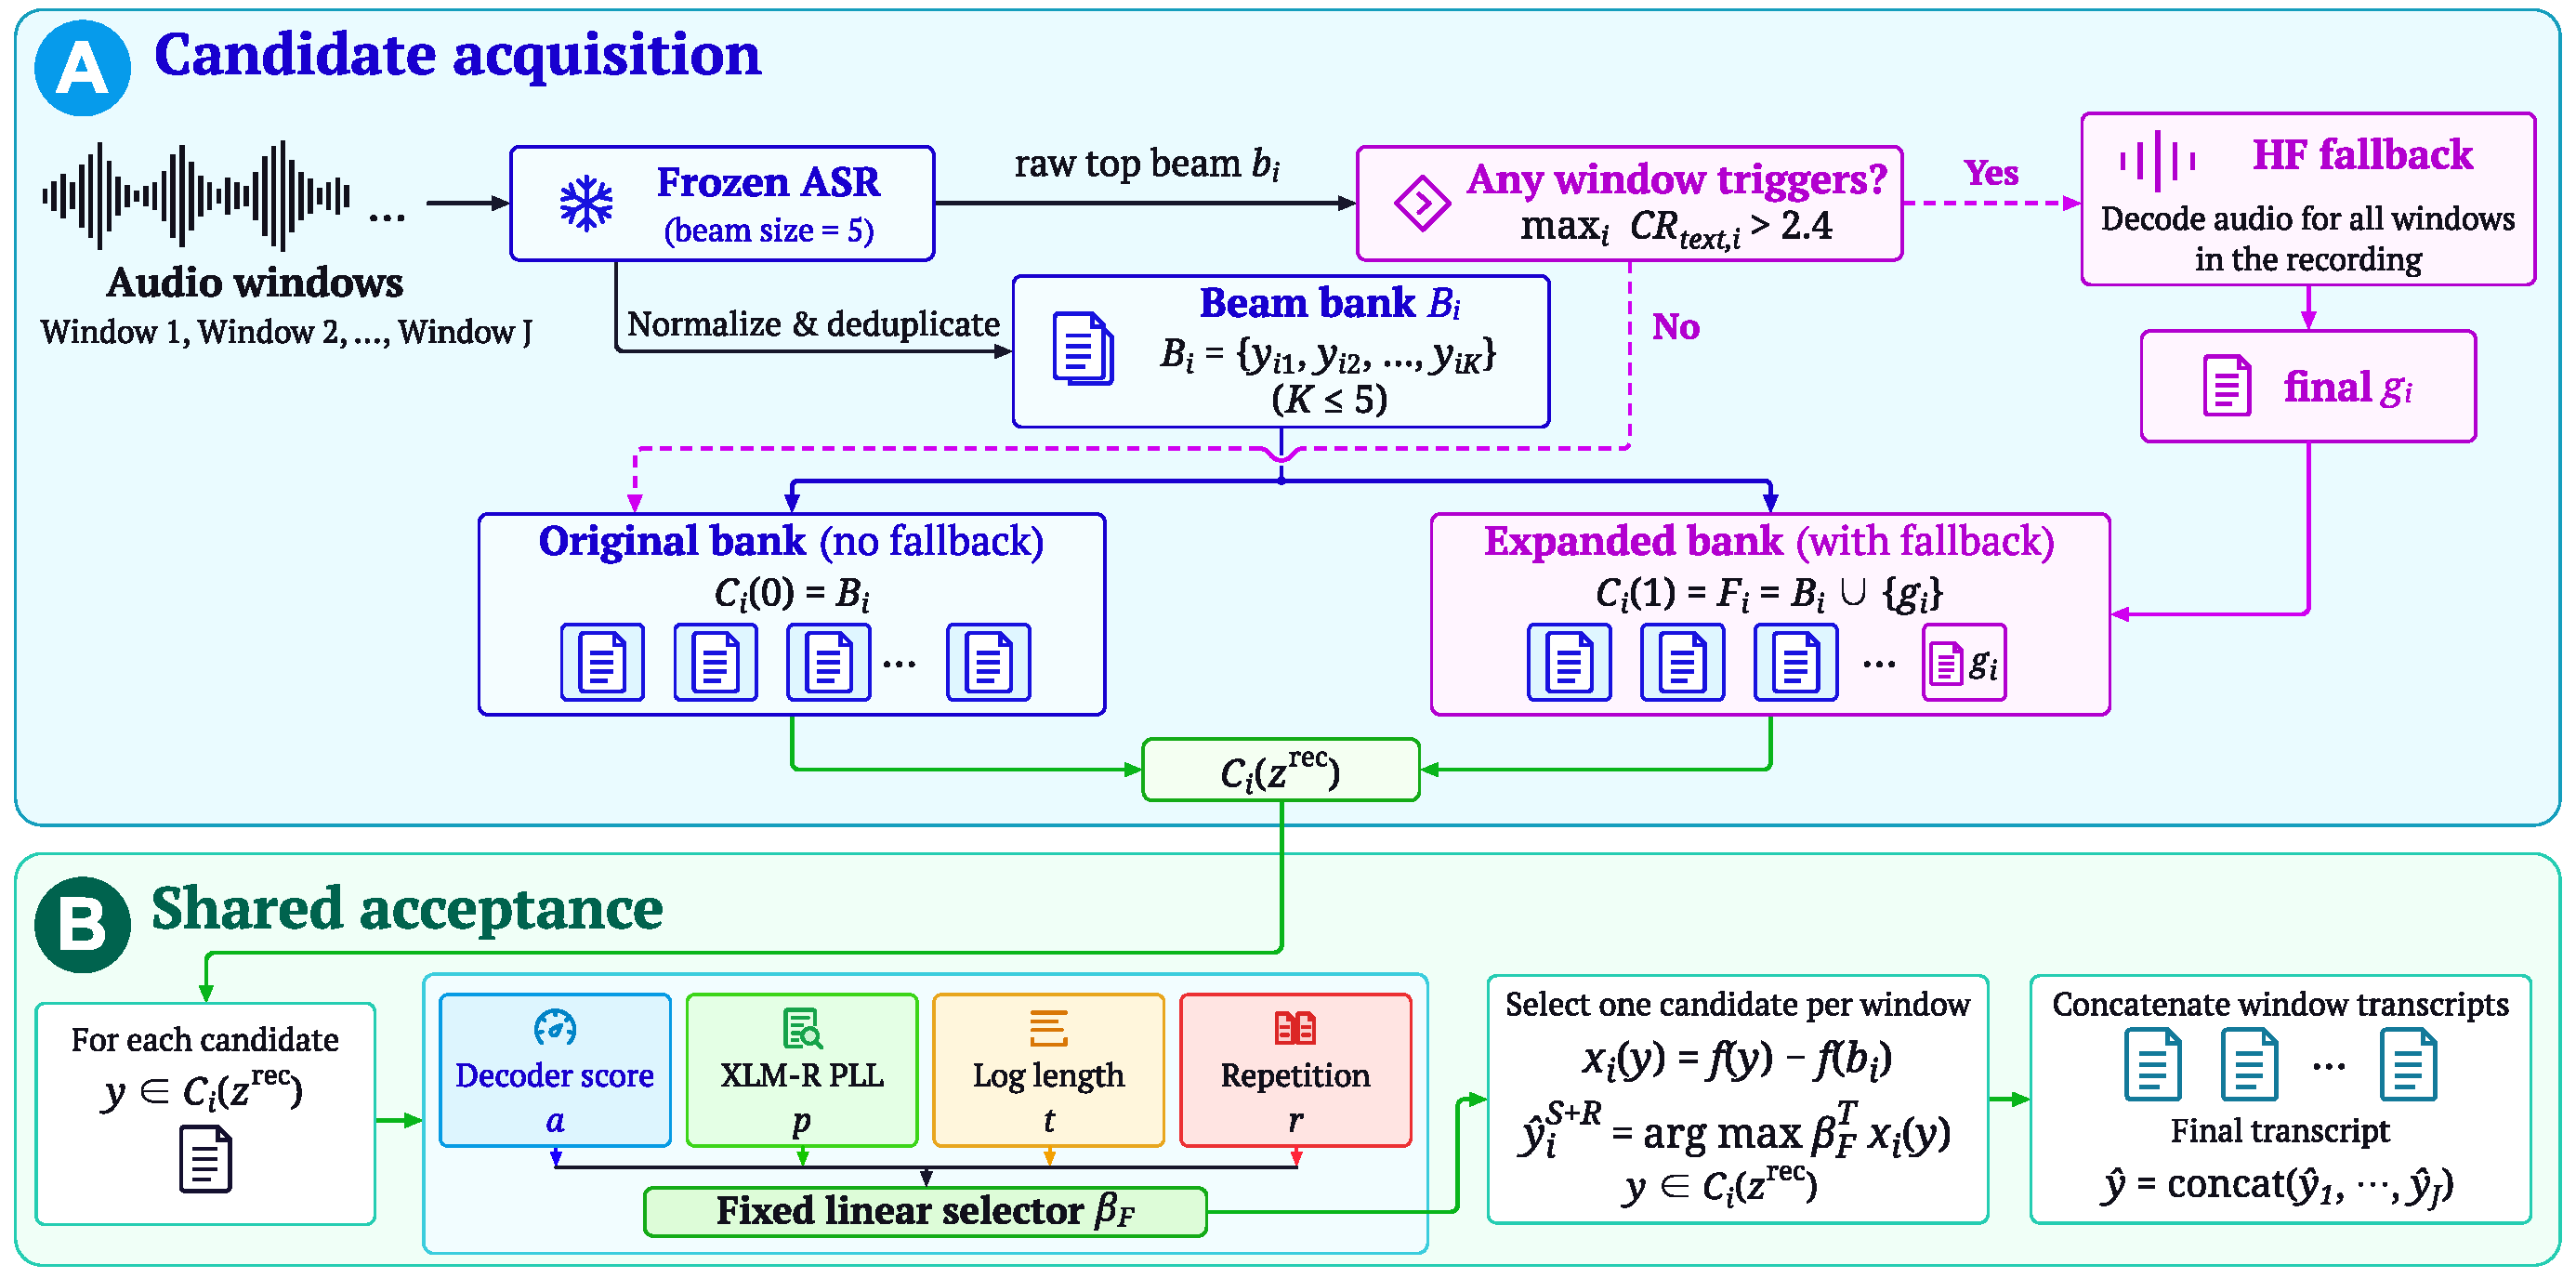
\includegraphics[width=0.64\textwidth]{figures/Figure1_Vector.pdf}
\caption{Acquisition (A) expands every window's candidate bank if any window triggers. Acceptance (B) applies the same fixed four-feature selector to the original or expanded bank. Selected window transcripts are then concatenated.}
\label{fig:workflow}\end{figure*}

\section{Controlled Acquisition and Acceptance}
\subsection{Recording-level acquisition}
We normalize and deduplicate five beams per window $i$ into $B_i$, retaining first occurrences and sources. With raw top beam $b_i$ and fallback $g_i$, $F_i=B_i\cup\{g_i\}$ contains at most six candidates. Before recovery, $\mathrm{CR}_{\mathrm{text}}$ divides top-beam UTF-8 byte length by zlib-compressed length, with zero for empty strings. The gate $z_i=\mathbf1\{\mathrm{CR}_{\mathrm{text},i}>2.4\}$ uses Whisper's standard text threshold~\cite{whisper}, fixed before confirmation. Recording-level invocation $z^{\mathrm{rec}}=\max_i z_i$ expands every window, even singletons (Fig.~\ref{fig:workflow}), as a conservative control. On single-window CV27 audio, $z^{\mathrm{rec}}=z_i$; Section~IV-D examines local routing for multi-window FLEURS.

Recovery follows Hugging Face temperatures $0,0.2,\ldots,1$ with compression, log-probability and no-speech thresholds $1.35$, $-1$ and $0.6$. The internal check compresses serialized token-ID bytes~\cite{hfwhisper4576} with a stricter retry threshold; the outer gate screens decoded text for severe loops. Shared leading bytes in two-byte Arabic/Persian characters can increase compression relative to ASCII Latin text at similar character repetition. Native HF uses the same retry configuration without N-best rescoring.

\subsection{Four-feature shared acceptance}
For features $f(y)=(a,p,t,r)$, $a$ is the mean teacher-forced log probability over $T$ body tokens without prefix, padding or end tokens, and $t=\log(1+T)$. XLM-R-base pseudo-log-likelihood $p$~\cite{xlmr,mlmscoring}, or PLL, averages individually masked nonspecial subword log probabilities in centered contexts of at most 510 subwords of the original string, rather than within-word masking~\cite{kauf2023}. Empty outputs have no body tokens or PLL targets and map to $f(\emptyset)=(0,0,0,0)$, but normalization alone need not yield zero features.

For normalized words $w_{1:M}$, the sequence-wide overlapping count is $c_y(u)=\sum_{k=1}^{M-n+1}\mathbf1\{w_{k:k+n-1}=u\}$. We measure repetition by
\begin{equation}
r_{n,h}(y)=\frac{\sum_{j=1}^{M-n+1}\mathbf1\{c_y(w_{j:j+n-1})\ge h\}}{\max(1,M-n+1)}.
\label{eq:repetition}
\end{equation}
We use $r(y)=r_{4,3}(y)$, which is zero for $M<4$. Repetitive sequences also motivate unlikelihood training~\cite{welleck2020}.

Centering $x_i(y)=f(y)-f(b_i)$ preserves rankings and softmax probabilities. Under fitted signs $(+,+,-,-)$, $\beta_F^\top f(y)<0=\beta_F^\top f(\emptyset)$ for every nonempty $y$, so any HF-proposed empty wins deterministically. For $x_{ik}=x_i(y_{ik})$, root-mean-square (RMS) scales satisfy $s_d^2=\sum_{\mathcal D}\omega_{ik}x_{ik,d}^2/\sum_{\mathcal D}\omega_{ik}$ over non-top training-fold pairs $\mathcal D=\{(i,k):i\in\bigcup_{\ell=1}^L\mathcal I_\ell,\ y_{ik}\in C_i\setminus\{b_i\}\}$. G4 uses $\omega_{ik}=1/[N_\ell(|C_i|-1)]$; all HF refits use $\omega_{ik}=1$. Scales below $10^{-12}$ become one. For reference $y_i^*$ and word-edit count $E$, define $\Delta_{ik}=E(b_i,y_i^*)-E(y_{ik},y_i^*)$ and $\pi_{ik}=\operatorname{softmax}_k\!\left(\theta^\top\operatorname{diag}(s)^{-1}x_{ik}\right)$. Both softmax and loss include all candidates, with $x_i(b_i)=\mathbf0$ and $\Delta_{i,b_i}=0$. Expected-risk fitting~\cite{mwer2018} minimizes
\begin{equation}
\mathcal L(\theta)=-\frac1L\sum_{\ell=1}^L\frac{\sum_{i\in\mathcal I_\ell}\sum_{k=1}^{|C_i|}\pi_{ik}\Delta_{ik}}{N_\ell}+\lambda\|\theta\|_2^2.
\label{eq:risk}
\end{equation}
Here $\mathcal I_\ell=\{i:\operatorname{lang}(i)=\ell\}$ indexes fitting windows, $N_\ell$ counts reference words and $L=5$.

The shared weights $\beta_F=\operatorname{diag}(s)^{-1}\theta$ are fitted per run on greedy-expanded DEV and fixed across sources, with ties broken by bank order. With $\hat{y}_i^B=\argmax_{y\in B_i}\beta_F^\top x_i(y)$, $C_i(0)=B_i$ and $C_i(1)=F_i$, the policies are
\begin{equation}
\begin{aligned}
\hat{y}_i^{S+R}&=\argmax_{y\in C_i(z^{\mathrm{rec}})}\beta_F^\top x_i(y),\\
\hat{y}_i^{\mathrm{Direct}}&=\begin{cases}\hat{y}_i^B,&z^{\mathrm{rec}}=0,\\g_i,&z^{\mathrm{rec}}=1.\end{cases}
\end{aligned}\label{eq:accept}
\end{equation}
Policy B reranks $B_i$, and N+R requests and reranks $F_i$ unconditionally. S+R and Direct share acquisition and use B off-trigger, but Direct bypasses selection and PLL on triggers. Window transcripts are concatenated for full-reference scoring.

\subsection{Matched acceptance controls}
G4 stays frozen. We fit H4 by expected risk on HF-expanded DEV banks and H3 without PLL, using $(a,t,r)$. RankNet~\cite{ranknet2005} minimizes
\begin{equation*}
\mathcal L_{\mathrm{rank}}=\frac1L\sum_{\ell=1}^L\frac{\sum_{i\in\mathcal I_\ell}\ell_i}{N_\ell}+\lambda\|\theta\|_2^2,
\end{equation*}
with $\ell_i=|\mathcal P_i|^{-1}\sum_{(j,k)\in\mathcal P_i}w_{jk}\log(1+e^{-\beta^\top(x_{ij}-x_{ik})})$ over unequal-edit pairs $\mathcal P_i=\{(j,k):E_j<E_k\}$, where $E_j=E(y_{ij},y_i^*)$ and $\beta=\operatorname{diag}(s)^{-1}\theta$. Empty $\mathcal P_i$ give $\ell_i=0$. HR4 uses $w_{jk}=1$; HWR4 uses $|E_j-E_k|/c$, with $c$ the training-fold mean gap under HR4's pair weights.

% Table I floats above the fitting discussion.
\begin{table}[!t]\centering\footnotesize
\caption{WER (\%) and pp contrasts before rounding. Checks denote HF acquisition, CR gating and R reselection ($\dagger$: off-trigger only).}\label{tab:paths}
\setlength{\tabcolsep}{2pt}\renewcommand{\arraystretch}{1.00}
\setlength{\abovecaptionskip}{3pt}
\setlength{\aboverulesep}{0.20ex}\setlength{\belowrulesep}{0.28ex}
\begin{tabular*}{\columnwidth}{@{\hspace{4pt}\extracolsep{\fill}}ccccccc@{\hspace{4pt}}}\toprule
Path & HF & CR & R & Scorer & \multicolumn{1}{c}{FLEURS} & \multicolumn{1}{c@{\hspace{4pt}}}{CV27}\\\midrule
Raw beam-5 top-1 & -- & -- & -- & -- & 18.90 & 36.41\\
Native HF~\cite{hfwhisper4576} & $\checkmark$ & -- & -- & -- & 18.55 & 33.80\\
B & -- & -- & $\checkmark$ & G4 & 17.45 & 33.98\\
N+R & $\checkmark$ & -- & $\checkmark$ & G4 & 17.09 & 31.68\\
S+R & $\checkmark$ & $\checkmark$ & $\checkmark$ & G4 & 17.09 & 31.68\\
Direct & $\checkmark$ & $\checkmark$ & $\checkmark^{\dagger}$ & G4 & 17.09 & 31.46\\
H3Direct & $\checkmark$ & $\checkmark$ & $\checkmark^{\dagger}$ & H3 & 18.68 & 33.64\\
\midrule\multicolumn{5}{l}{\bfseries A. TEST oracle bounds} & \multicolumn{1}{c}{FLEURS} & \multicolumn{1}{c@{\hspace{4pt}}}{CV27}\\
\multicolumn{5}{c}{Original-bank oracle} & 16.19 & 30.19\\
\multicolumn{5}{c}{Full-HF oracle} & 15.83 & 27.68\\
\multicolumn{5}{c}{CR-routed oracle} & 15.83 & 27.68\\
\multicolumn{5}{c}{S+R gap to routed oracle, pp} & 1.26 & 4.00\\
\end{tabular*}\par\nointerlineskip
\begin{tabular*}{\columnwidth}{@{\hspace{4pt}\extracolsep{\fill}}cccc@{\hspace{4pt}}}
\midrule\multicolumn{4}{l}{\bfseries B. Locked CV27 confirmation (7,500 recordings)}\\
 & \multicolumn{1}{c}{B} & \multicolumn{1}{c}{N+R = S+R} & \multicolumn{1}{c@{\hspace{4pt}}}{Gain}\\\midrule
Macro-average & 35.02 & 32.75 & 2.26\\
\end{tabular*}\par\nointerlineskip
\begin{tabular*}{\columnwidth}{@{\hspace{4pt}\extracolsep{\fill}}ccc@{\hspace{4pt}}}
\midrule Contrast & \multicolumn{1}{c}{$\Delta$WER (pp)} & \multicolumn{1}{c@{\hspace{4pt}}}{95\% upper bound (pp)}\\
S+R $-$ B & -2.26 & -1.32\\
S+R $-$ N+R & 0.00 & 0.00\\
\bottomrule\end{tabular*}\end{table}

Connected clients and reference texts define five folds per language. Held-fold macro WER selects among 49 log-spaced penalties from $10^{-4}$ to $1$, preferring larger values on ties. L-BFGS-B refits full DEV from zero. Singletons enter WER denominators, and padding is excluded.

MBR~\cite{goel2000mbr} selects $\hat y_i=\allowbreak\argmin_{y\in C_i}\sum_{y'\in C_i}q_i(y')E(y,y')$. U-MBR uses $q_i(y')\propto1$ and D-MBR uses $q_i(y')=\operatorname{softmax}(Ta/\tau)_{y'}$. DEV WER selects $\tau\in\{0.1,0.3,1,3,10\}$, favoring larger values on ties; candidate ties retain bank order. \emph{Complete} policies use each acceptor on both banks; \emph{triggered} comparisons keep G4 off-trigger with full-panel denominators.

\section{Data and Evaluation}
We adapt Whisper-small~\cite{whisper} on 44.60~h of FLEURS TRAIN~\cite{fleurs} across Arabic, Persian, Polish, Turkish and Italian using LoRA~\cite{lora} over three random seeds (4,656 updates, rank and scale four, zero dropout across all attention projections). LoRA sees no CV27 data, so CV27 tests zero-shot acoustic transfer across domains. Selectors do use CV27 DEV, where recovery was checked with the fixed gate before confirmation. Evaluation on FLEURS TEST (13.07~h; 3,665 recordings) and CV27 TEST (83.00~h; 58,514 recordings)~\cite{cv2020} is retrospective because both splits were accessed during development.

The locked confirmation panel has 7,500 CV27 TRAIN recordings (1,500 per language) with no previously accessed audio or reference texts. Predictions, stopping rules and the one-sided 0.10\,pp noninferiority margin were locked before reference evaluation. We use 10,000 synchronized bootstrap draws of speaker components within languages. Speakers recurring across splits limit generalization to this sampling frame. Confirmation covers the original G4 acquisition policy; later gates, refits and window policies remain retrospective.

We weight costs by inverse sampling probabilities for 255 FLEURS and 472 CV27 recordings. The sample covers all first-checkpoint triggers or Native HF output changes and ten ordinary recordings per language and duration quintile. Study~A measures four paths across three checkpoints; Study~B measures seven on one. Later-checkpoint omissions comprise five FLEURS and 207 CV27 triggers (0.05\% and 0.12\% of seed--recordings). Triggered N+R and S+R execute identical operations, though sampling shares do not bound timing variation. Study~B covers all its triggers and corroborates Study~A's savings (5.18\% and 4.54\% versus 5.15\% and 4.57\%). Both use three randomized paired rounds with each recording block on one of four NVIDIA A40 (48~GB) GPUs, resident models, within-path encoder and first-search reuse, and 32-mask PLL batches. Waveform-to-output timing excludes loading, warmup and interfered blocks. Peak CUDA memory is the maximum per-process allocation in MiB over calls and rounds. Session-conditional intervals use 4,000 paired stratified draws with finite-population correction; Study~A averages checkpoints with synchronized draws.

Known-language decoding uses bfloat16, five beams, length penalty one, native suppression and a 444-token cap in Transformers 4.57.6. At 16\,kHz, $N$ samples give $J=\lceil N/480000\rceil$ windows bounded by $\lfloor jN/J\rfloor$ without previous-window text. Deduplication, WER and $r$ share NFC normalization, digit unification, punctuation-to-space, Persian mapping and Turkish casing~\cite{normalization}, with fixed source RNG mappings. WER averages five language aggregates and three seeds; calls pool seed--recordings. TEST intervals use 2,000 paired client/reference-component draws within languages, synchronized across seeds with fits and source draws frozen. FLEURS comparisons are descriptive because component metadata are unverified.



\begin{table}[!b]\centering\footnotesize
\caption{Same-HF TEST WER (\%) and gain B$-$S (pp) before rounding. Checks denote PLL, pairwise P and edit-gap weighting W.}\label{tab:hfacceptors}
\setlength{\tabcolsep}{1.6pt}\renewcommand{\arraystretch}{1.00}
\begin{tabular*}{\columnwidth}{@{\hspace{4pt}\extracolsep{\fill}}cccccccccc@{\hspace{4pt}}}\toprule
\multirow{2}{*}[-0.6ex]{Acceptor} & \multirow{2}{*}[-0.6ex]{PLL} & \multirow{2}{*}[-0.6ex]{P} & \multirow{2}{*}[-0.6ex]{W} & \multicolumn{3}{c}{FLEURS} & \multicolumn{3}{c}{CV27}\\
\cmidrule(l{0.2em}r{0.2em}){5-7}\cmidrule(l{0.2em}r{0.2em}){8-10}
 & & & & \multicolumn{1}{c}{B} & \multicolumn{1}{c}{S} & \multicolumn{1}{c}{Gain} & \multicolumn{1}{c}{B} & \multicolumn{1}{c}{S} & \multicolumn{1}{c@{\hspace{4pt}}}{Gain}\\\midrule
G4~\cite{mwer2018} & $\checkmark$ & -- & -- & 17.45 & 17.09 & 0.37 & 33.98 & 31.68 & 2.30\\
H4~\cite{mwer2018} & $\checkmark$ & -- & -- & 17.46 & 17.09 & 0.37 & 33.97 & 31.52 & 2.45\\
HR4~\cite{ranknet2005} & $\checkmark$ & $\checkmark$ & -- & 17.51 & 17.14 & 0.37 & 34.02 & 32.30 & 1.72\\
H3~\cite{mwer2018} & -- & -- & -- & 19.05 & 18.68 & 0.37 & 36.15 & 33.77 & 2.38\\
HWR4~\cite{ranknet2005} & $\checkmark$ & $\checkmark$ & $\checkmark$ & 17.47 & 17.10 & 0.37 & 33.97 & 31.44 & 2.53\\
U-MBR~\cite{goel2000mbr} & -- & -- & -- & 19.14 & 19.14 & 0.00 & 36.91 & 36.88 & 0.03\\
D-MBR~\cite{goel2000mbr} & -- & -- & -- & 18.92 & 18.75 & 0.17 & 36.09 & 34.48 & 1.60\\
\end{tabular*}\par\nointerlineskip
\begin{tabular*}{\columnwidth}{@{\hspace{4pt}\extracolsep{\fill}}ccc@{\hspace{4pt}}}
\midrule\multicolumn{3}{c}{\itshape A. Original family: CV27 $\Delta$WER (individual 97.5\% CI)}\\
Triggered HR4 $-$ H4 & +0.72 & [+0.40, +1.16]\\
Complete H3 $-$ H4 & +2.25 & [+2.16, +2.34]\\
\addlinespace[1pt]\multicolumn{3}{c}{\itshape B. Later two-comparison family}\\
Triggered U-MBR $-$ H4 & +2.51 & [+1.93, +3.18]\\
Triggered HWR4 $-$ H4 & -0.08 & [-0.15, -0.03]\\
\bottomrule\end{tabular*}\end{table}

\section{Results}
\subsection{Acquisition with fixed acceptance}
On the locked confirmation panel, S+R gains 2.26\,pp over B, with seed gains of 0.20 to 4.54\,pp (Table~\ref{tab:paths}). Matching N+R's error counts in every seed meets the prespecified 0.10\,pp margin but does not guarantee zero loss under distribution shift. Of 61 triggers, 49 improve edits and two worsen them.

Retrospective evaluation yields 32.71\% WER for Direct versus S+R's locked 32.75\%. Both beat B and Native HF's retrospective 34.87\% by over 2.1\,pp. Direct's unrounded difference from S+R is $-0.05$\,pp with a paired speaker-bootstrap 95\% interval from $-0.19$ to $+0.04$\,pp.

On TEST, S+R retains all ten beneficial FLEURS instances at 0.09\% calls and 370 of 373 CV27 instances at 0.30\%, with five edits missed. We obtain 99.98\% retention by dividing retained positive edit gain by available gain after normalizing both by full language reference counts and averaging over languages and seeds. Normalized N+R and S+R outputs differ on one FLEURS and 13 CV27 nontriggers despite nearly identical WER. Reference-assisted oracles minimize recording edits after window concatenation over original, expanded or CR-routed banks. Routing changes this bound by under 0.01\,pp versus CV27 S+R's 4.00\,pp gap, so acceptance offers greater headroom.

\subsection{Interaction with the fallback source}
S+R can reject unscreened fallbacks and beats Direct by 0.53\,pp with greedy recovery and 0.43\,pp with one $T=0.2$ draw. HF screens retries internally, but G4 was fitted on greedy expansions. Direct then leads by 0.22\,pp, with a 95\% interval from 0.11 to 0.37\,pp. The gain comes from one checkpoint ($-0.68$\,pp versus $+0.00$ and $+0.02$\,pp). DEV favored HF reselection at 30.08\% versus 30.09\% and guided the fixed acquisition control.

Direct retains 67.13\% of positive gain from unconditional final HF, compared with S+R's 99.98\% from N+R. Relative to its own control, Direct forgoes 1.24\,pp of benefit but avoids 3.58\,pp of harm.

\begin{table}[!t]\centering\footnotesize
\caption{Population-weighted ms and observed peak allocated MiB with both models resident. Each study uses three paired rounds.}\label{tab:cost}
\setlength{\tabcolsep}{3pt}\renewcommand{\arraystretch}{1.00}
% Balance the added group rules within the existing table height.
\setlength{\aboverulesep}{0.3ex}\setlength{\belowrulesep}{0.45ex}
\begin{tabular*}{\columnwidth}{@{\hspace{4pt}\extracolsep{\fill}}ccccc@{\hspace{4pt}}}\toprule
\multirow{2}{*}[-0.5ex]{Path} & \multicolumn{2}{c}{FLEURS} & \multicolumn{2}{c}{CV27}\\
\cmidrule(l{0.2em}r{0.2em}){2-3}\cmidrule(l{0.2em}r{0.2em}){4-5}
 & \multicolumn{1}{c}{ms} & \multicolumn{1}{c}{MiB} & \multicolumn{1}{c}{ms} & \multicolumn{1}{c@{\hspace{4pt}}}{MiB}\\\midrule
\multicolumn{5}{c}{\itshape A. Four-path comparison across three checkpoints}\\
Native HF & 1291.7 & 2980.8 & 517.4 & 2813.8\\
B & 1352.7 & 3144.9 & 591.9 & 3133.1\\
N+R & 1436.8 & 2988.3 & 639.2 & 3133.1\\
S+R & 1362.8 & 3189.7 & 610.0 & 3133.1\\
\midrule
\multicolumn{5}{c}{\itshape B. Seven-path comparison on one checkpoint}\\
Native HF & 1304.8 & 2978.4 & 531.2 & 2811.8\\
Raw top-1 & 1222.6 & 2946.6 & 479.9 & 2571.0\\
B & 1364.0 & 3142.4 & 605.1 & 3131.1\\
N+R & 1449.6 & 2986.3 & 657.9 & 3131.1\\
S+R & 1374.5 & 3187.2 & 628.0 & 3131.1\\
Direct & 1372.8 & 3187.2 & 625.8 & 2811.8\\
H3Direct & 1314.0 & 3187.2 & 586.4 & 2811.8\\
\midrule
\multicolumn{5}{c}{\itshape Relative latency saving: S+R versus N+R (95\% CI)}\\
Study A & \multicolumn{2}{c}{5.15\% [2.84, 9.41]} & \multicolumn{2}{c}{4.57\% [4.40, 4.73]}\\
Study B & \multicolumn{2}{c}{5.18\% [2.88, 9.39]} & \multicolumn{2}{c}{4.54\% [4.44, 4.66]}\\
\midrule
\multicolumn{5}{c}{\itshape Matched-study B-path increments}\\
B $-$ Raw top-1, ms & \multicolumn{2}{c}{141.4} & \multicolumn{2}{c}{125.2}\\
N+R $-$ B, ms & \multicolumn{2}{c}{85.6} & \multicolumn{2}{c}{52.8}\\
S+R $-$ B, ms & \multicolumn{2}{c}{10.5} & \multicolumn{2}{c}{22.9}\\
Fallback increment saved & \multicolumn{2}{c}{87.7\%} & \multicolumn{2}{c}{56.6\%}\\
\bottomrule\end{tabular*}\end{table}

\subsection{Acceptance on matched HF banks}
After refitting on HF banks, H4 improves over G4 but trails Direct. Weighted HWR4 yields the lowest complete CV27 WER of 31.44\% (Table~\ref{tab:hfacceptors}, where S denotes each acceptor's selective policy). Triggered HR4 trails H4 in every seed ($+0.91$, $+0.08$ and $+1.17$\,pp). Edit-gap weighting reverses the mean contrast to $-0.08$\,pp through a 0.25\,pp gain in one checkpoint. Intervals provide 95\% Bonferroni coverage per family, with 10,000 synchronized draws for the later family.

FLEURS gains round to 0.37\,pp for fitted acceptors because S equals its own B off-trigger. H3's B has two fewer errors on one of ten triggers, but S errors match and the average difference is below 0.006\,pp. Nontriggers account for 97.23\% of the refitted H3--H4 WER gap in routine selection, without isolating PLL's causal contribution or time share.

\subsection{Cost, heterogeneity and supporting diagnostics}
For systems using B, S+R preserves N+R's accuracy gain at lower recovery overhead (Table~\ref{tab:cost}). In Study B, B exceeds raw top-1 by 141.4\,ms on FLEURS and 125.2\,ms on CV27. S+R saves 87.7\% and 56.6\% of N+R's increment over B. An unweighted CV27 profile of 25 recordings averages teacher scoring at 85.9\,ms and PLL at 149.3\,ms, with both stages skipped for two singletons. The larger population share of singletons explains the smaller overall increment; stage shares were not measured separately. Native HF skips N-best rescoring and is faster at a WER cost of 1.46\,pp on FLEURS and over 2.1\,pp on CV27 TEST.

H3Direct uses H3 off-trigger and final HF on triggers, and omits PLL like raw top-1. On CV27 it saves 6.29\% over Direct but trails Native HF by 55.2\,ms, with a 95\% interval of 52.3 to 58.2\,ms; the FLEURS interval spans zero.
H4 and HWR4 only replace G4's weights; selective PLL remains future work. In Study B, Direct bypasses scoring on the CV27 trigger responsible for B's peak CUDA memory. On FLEURS, Direct and H3Direct match S+R's peak CUDA allocation during the same two-window recovery, with both windows' state retained.

\begin{table}[t]\centering\footnotesize
\caption{TEST gains averaged over seeds. Calls pool seed--recordings.}\label{tab:language}
\setlength{\tabcolsep}{3pt}\renewcommand{\arraystretch}{1.00}
\begin{tabular*}{\columnwidth}{@{\hspace{4pt}\extracolsep{\fill}}ccccc@{\hspace{4pt}}}\toprule
\multirow{2}{*}[-0.6ex]{Language} & \multicolumn{2}{c}{FLEURS} & \multicolumn{2}{c}{CV27}\\
\cmidrule(l{0.2em}r{0.2em}){2-3}\cmidrule(l{0.2em}r{0.2em}){4-5}
 & Calls, \% & Gain, pp & Calls, \% & \multicolumn{1}{c@{\hspace{4pt}}}{Gain, pp}\\\midrule
Arabic & 0.23 & 0.64 & 0.11 & 1.40\\
Persian & 0.27 & 1.20 & 1.15 & 9.05\\
Polish & 0.00 & 0.00 & 0.33 & 0.30\\
Turkish & 0.00 & 0.00 & 0.03 & 0.51\\
Italian & 0.00 & 0.00 & 0.02 & 0.23\\
\end{tabular*}\par\nointerlineskip
\begin{tabular*}{\columnwidth}{@{\hspace{4pt}\extracolsep{\fill}}cccc@{\hspace{4pt}}}
\midrule\multicolumn{4}{c}{\itshape Empty-HF acceptance diagnostic (18 instances, 11 recordings)}\\
Acceptance minus B reversion & $S=-118$ & $D=+120$ & $I=-1995$\\
\bottomrule\end{tabular*}\end{table}

Empty TEST candidates enter only through HF. Under signs $(+,+,-,-)$, the centered abstention baseline in Section~II-B outranks candidates with $a,p\le0$, $t>0$ and $r\ge0$, even without repetition. Accepting 18 empties in 11 CV27 recordings removes 1,995 insertions, with S/D/I tradeoffs in Table~\ref{tab:language}. This accords with hallucination suppression~\cite{baranski2025nonspeech}, although silence labels are needed to establish acoustic causes. Reverting these acceptances to B retains 91.52\% of gain, or 2.10\,pp at 31.88\% WER. The H4+$e$ refit adds $e(y)=\mathbf1\{y=\emptyset\}$ on H4's DEV folds and grid and retains all 18 acceptances at 31.52\% WER. These acceptances agree with the aggregate benefit, but only one or two DEV empties per checkpoint limit calibration.

The change from raw top-1 to B measures routine rescoring across five languages; B to S+R isolates sparse repetition recovery. Persian contributes 78.77\% of CV27 TEST gain and 84.07\% of gain on the locked confirmation panel (Table~\ref{tab:language}). Excluding Persian, the four-language macro gain remains 0.61\,pp on CV27 TEST and 0.45\,pp on the locked confirmation panel. Polish, Turkish and Italian have no FLEURS triggers or gains. These patterns track repetition without separating script, acoustics or LoRA effects. The 22 two-window FLEURS recordings yield 52.69\% of net gain. On cached TEST banks, local S+R routing reduces window requests from 15 to 10 with unchanged error counts. Local Direct changes WER by under 0.01\,pp, although live request order may alter RNG draws.

\raggedbottom
\section{Conclusion}
On the locked panel, selective acquisition matches unconditional recovery across seeds. Separate timing studies show lower recovery cost. Retrospective controls favor expected risk over unweighted ranking on matched HF banks in every seed.

Acceptance should reflect fallback screening. Direct skips trigger-time rescoring of screened HF outputs with comparable accuracy; unscreened draws benefit from reselection. HWR4 has the lowest exploratory CV27 WER, but its advantage over H4 is concentrated in one checkpoint. Future work includes script-normalized gates, window-local routing and confidence-gated PLL.
\section*{Acknowledgment}
Supported by the National Natural Science Foundation of China under Grant 62466058 and Autonomous Region Key R\&D Program under Grant 2025B03042-1.
\label{iscas:body-end}\clearpage\raggedbottom\balance
\label{iscas:references-start}
% IEEEtran bibliography style; verified entries manually maintained.
\begin{thebibliography}{99}
% Keep each bibliographic entry intact when balancing the final two columns.
\interlinepenalty=10000
\providecommand{\url}[1]{#1}
\csname url@samestyle\endcsname
\providecommand{\newblock}{\relax}
\providecommand{\bibinfo}[2]{#2}
\providecommand{\BIBentrySTDinterwordspacing}{\spaceskip=0pt\relax}
\providecommand{\BIBentryALTinterwordstretchfactor}{4}
\providecommand{\BIBentryALTinterwordspacing}{\spaceskip=\fontdimen2\font plus
\BIBentryALTinterwordstretchfactor\fontdimen3\font minus \fontdimen4\font\relax}
\providecommand{\BIBforeignlanguage}[2]{{%
\expandafter\ifx\csname l@#1\endcsname\relax
\typeout{** WARNING: IEEEtran.bst: No hyphenation pattern has been}%
\typeout{** loaded for the language `#1'. Using the pattern for}%
\typeout{** the default language instead.}%
\else
\language=\csname l@#1\endcsname
\fi
#2}}
\providecommand{\BIBdecl}{\relax}
\BIBdecl

\bibitem{gaur2022}
N.~Gaur, T.~Chen, E.~Variani, P.~Haghani, B.~Ramabhadran, and P.~J. Moreno, ``{Multilingual second-pass rescoring for automatic speech recognition systems},'' in \emph{Proceedings of the IEEE International Conference on Acoustics, Speech and Signal Processing}, 2022, pp. 6407--6411.
\bibitem{yan2025wild}
B.~Yan, V.~Pratap, S.~Watanabe, and M.~Auli, ``{Improving multilingual ASR in the wild using simple N-best re-ranking},'' in \emph{Proceedings of the IEEE International Conference on Acoustics, Speech and Signal Processing}, 2025, pp. 1--5.
\bibitem{rescorebert}
L.~Xu \emph{et~al.}, ``{RescoreBERT: Discriminative speech recognition rescoring with BERT},'' in \emph{Proceedings of the IEEE International Conference on Acoustics, Speech and Signal Processing}, 2022, pp. 6117--6121.
\bibitem{discriminative2023}
P.~G. Shivakumar, J.~Kolehmainen, Y.~Gu, A.~Gandhe, A.~Rastrow, and I.~Bulyko, ``{Discriminative speech recognition rescoring with pre-trained language models},'' in \emph{Proceedings of the IEEE Automatic Speech Recognition and Understanding Workshop}, 2023, pp. 1--7.
\bibitem{audioattention2019}
A.~Gandhe and A.~Rastrow, ``{Audio-attention discriminative language model for ASR rescoring},'' in \emph{Proceedings of the IEEE International Conference on Acoustics, Speech and Signal Processing}, 2020, pp. 7944--7948.
\bibitem{fiscus1997} J.~G. Fiscus, ``A post-processing system to yield reduced word error rates: Recognizer output voting error reduction (ROVER),'' in \emph{Proceedings of the IEEE Automatic Speech Recognition and Understanding Workshop}, 1997, pp. 347--354.
\bibitem{mangu2000} L.~Mangu, E.~Brill, and A.~Stolcke, ``Finding consensus in speech recognition: Word error minimization and other applications of confusion networks,'' \emph{Computer Speech and Language}, vol.~14, no.~4, pp. 373--400, 2000.
\bibitem{kuo2026framework}
C.-H. Kuo and K.-Y. Chen, ``{An integrated framework for ASR post-processing with error correction, rescoring, and text-speech matching},'' \emph{APSIPA Transactions on Signal and Information Processing}, vol.~15, no.~1, pp. 223--248, 2026, doi: \href{https://doi.org/10.1108/ATSIP-07-2025-0069}{\nolinkurl{10.1108/ATSIP-07-2025-0069}}.
\bibitem{dutta2022}
S.~Dutta, S.~Jain, A.~Maheshwari, S.~Pal, G.~Ramakrishnan, and P.~Jyothi, ``{Error correction in ASR using sequence-to-sequence models},'' arXiv:2202.01157, 2022.
\bibitem{progres2024}
A.~D. Tur, A.~Moumen, and M.~Ravanelli, ``{ProGRes: Prompted generative rescoring on ASR N-best},'' in \emph{Proceedings of the IEEE Spoken Language Technology Workshop}, 2024, pp. 600--607, doi: \href{https://doi.org/10.1109/slt61566.2024.10832194}{\nolinkurl{10.1109/slt61566.2024.10832194}}.
\bibitem{whisperingllama}
S.~Radhakrishnan, C.-H. Yang, S.~Khan, R.~Kumar, N.~Kiani, D.~Gomez-Cabrero, and J.~Tegnér, ``{Whispering LLaMA: A cross-modal generative error correction framework for speech recognition},'' in \emph{Proceedings of the Conference on Empirical Methods in Natural Language Processing}, 2023, pp. 10007--10016, doi: \href{https://doi.org/10.18653/v1/2023.emnlp-main.618}{\nolinkurl{10.18653/v1/2023.emnlp-main.618}}.
\bibitem{cheng2023pruning}
J. Cheng and A. Vlachos, ``Faster minimum Bayes risk decoding with confidence-based pruning,'' in \emph{Proceedings of the 2023 Conference on Empirical Methods in Natural Language Processing}, 2023, pp. 12473--12480, doi: \href{https://doi.org/10.18653/v1/2023.emnlp-main.767}{\nolinkurl{10.18653/v1/2023.emnlp-main.767}}.
\bibitem{jinnai2025mbrasr}
\BIBentryALTinterwordspacing
Y.~Jinnai, ``Re-evaluating minimum Bayes risk decoding for automated speech recognition tasks,'' \emph{Transactions on Machine Learning Research}, 2026. [Online]. Available: \url{https://openreview.net/forum?id=I6iLWhRIsf}.
\BIBentrySTDinterwordspacing
\bibitem{xue2025sima}
H.~Xue, Y.~Tang, J.~Zhang, X.~Geng, and L.~Xie, ``{Selective invocation for multilingual ASR: A cost-effective approach adapting to speech recognition difficulty},'' in \emph{Proceedings of Interspeech}, 2025, pp. 2580--2584, doi: \href{https://doi.org/10.21437/interspeech.2025-1652}{\nolinkurl{10.21437/interspeech.2025-1652}}.
\bibitem{aleksic2025}
P.~Aleksic and L.~Zhou, ``Latency reduction in conversational user interfaces by selective execution of multi-pass speech recognition based on LLM evaluation,'' \emph{Technical Disclosure Commons}, technical disclosure, Jun.~27, 2025. [Online]. Available: \url{https://www.tdcommons.org/dpubs_series/8287/}.
\bibitem{fathullah2024proxies}
Y.~Fathullah, P.~Radmard, A.~Liusie, and M.~Gales, ``Who needs decoders? Efficient estimation of sequence-level attributes with proxies,'' in \emph{Proceedings of the 18th Conference of the European Chapter of the Association for Computational Linguistics}, 2024, pp. 1478--1496, doi: \href{https://doi.org/10.18653/v1/2024.eacl-long.89}{\nolinkurl{10.18653/v1/2024.eacl-long.89}}.
\bibitem{lim2025hybrid}
Y.~Lim, J.~Park, H.~Y. Kim, H.~Lee, and B.-Y. Kim, ``Hybrid decoding: Rapid pass and selective detailed correction for sequence models,'' in \emph{Proceedings of the IEEE Automatic Speech Recognition and Understanding Workshop}, 2025, pp. 1--7, doi: \nolinkurl{10.1109/ASRU65441.2025.11434678}.
\bibitem{ferraz2024distil}
T.~P. Ferraz, M.~Zanon Boito, C.~Brun, and V.~Nikoulina, ``Multilingual DistilWhisper: Efficient distillation of multi-task speech models via language-specific experts,'' in \emph{Proceedings of the IEEE International Conference on Acoustics, Speech and Signal Processing}, 2024, pp. 10716--10720, doi: \nolinkurl{10.1109/ICASSP48485.2024.10447520}.
\bibitem{jitkrittum2023cascade} W. Jitkrittum, N. Gupta, A. K. Menon, H. Narasimhan, A. S. Rawat, and S. Kumar, ``When does confidence-based cascade deferral suffice?,'' in \textit{Advances in Neural Information Processing Systems}, vol. 36, 2023, doi: 10.52202/075280-0431.
\bibitem{mwer2018}
R.~Prabhavalkar \emph{et~al.}, ``{Minimum word error rate training for attention-based sequence-to-sequence models},'' in \emph{Proceedings of the IEEE International Conference on Acoustics, Speech and Signal Processing}, 2018, pp. 4839--4843.
\bibitem{ranknet2005}
C.~Burges \emph{et~al.}, ``{Learning to rank using gradient descent},'' in \emph{Proceedings of the 22nd International Conference on Machine Learning}, 2005, pp. 89--96.
\bibitem{goel2000mbr}
V.~Goel and W.~J. Byrne, ``{Minimum Bayes-risk automatic speech recognition},'' \emph{Computer Speech and Language}, vol.~14, no.~2, pp. 115--135, Apr. 2000.
\bibitem{hfwhisper4576}
Hugging Face, ``Whisper generation implementation,'' \emph{Transformers}, v4.57.6, documentation and \texttt{\_retrieve\_compression\_ratio}. [Online]. Available: \url{https://github.com/huggingface/transformers/blob/v4.57.6/src/transformers/models/whisper/generation_whisper.py}
\bibitem{xlmr}
A.~Conneau \emph{et~al.}, ``{Unsupervised cross-lingual representation learning at scale},'' in \emph{Proceedings of the 58th Annual Meeting of the Association for Computational Linguistics}, 2020, pp. 8440--8451.
\bibitem{mlmscoring}
J.~Salazar, D.~Liang, T.~Q. Nguyen, and K.~Kirchhoff, ``{Masked language model scoring},'' in \emph{Proceedings of the 58th Annual Meeting of the Association for Computational Linguistics}, 2020, pp. 2699--2712.
\bibitem{kauf2023}
C.~Kauf and A.~Ivanova, ``{A better way to do masked language model scoring},'' in \emph{Proceedings of the 61st Annual Meeting of the Association for Computational Linguistics, Vol. 2: Short Papers}, 2023, pp. 925--935.
\bibitem{welleck2020}
\BIBentryALTinterwordspacing
S.~Welleck, I.~Kulikov, S.~Roller, E.~Dinan, K.~Cho, and J.~Weston, ``{Neural text generation with unlikelihood training},'' in \emph{Proceedings of the International Conference on Learning Representations}, 2020.
\BIBentrySTDinterwordspacing
\bibitem{fleurs}
\BIBentryALTinterwordspacing
A.~Conneau \emph{et~al.}, ``{FLEURS: Few-shot learning evaluation of universal representations of speech},'' in \emph{Proceedings of the IEEE Spoken Language Technology Workshop}, 2023, pp. 798--805. [Online]. Available: \url{https://huggingface.co/datasets/google/fleurs}.
\BIBentrySTDinterwordspacing
\bibitem{whisper}
\BIBentryALTinterwordspacing
A.~Radford, J.~W. Kim, T.~Xu, G.~Brockman, C.~McLeavey, and I.~Sutskever, ``{Robust speech recognition via large-scale weak supervision},'' in \emph{Proceedings of the 40th International Conference on Machine Learning}, ser. Proceedings of Machine Learning Research, vol. 202, 2023, pp. 28\,492--28\,518. [Online]. Available: \url{https://proceedings.mlr.press/v202/radford23a.html}.
\BIBentrySTDinterwordspacing
\bibitem{lora}
\BIBentryALTinterwordspacing
E.~J. Hu \emph{et~al.}, ``{LoRA: Low-rank adaptation of large language models},'' in \emph{Proceedings of the International Conference on Learning Representations}, 2022. [Online]. Available: \url{https://openreview.net/forum?id=nZeVKeeFYf9}.
\BIBentrySTDinterwordspacing
\bibitem{cv2020}
R.~Ardila \emph{et~al.}, ``Common Voice: A massively-multilingual speech corpus,'' in \emph{Proceedings of the Twelfth Language Resources and Evaluation Conference}, 2020, pp. 4218--4222. [Online]. Available: \url{https://aclanthology.org/2020.lrec-1.520/}.
\bibitem{normalization}
K.~Manohar and L.~G. Pillai, ``{What is lost in normalization? Exploring pitfalls in multilingual ASR model evaluations},'' in \emph{Proceedings of the Conference on Empirical Methods in Natural Language Processing}, 2024, pp. 10\,864--10\,869.
\bibitem{baranski2025nonspeech} M. Bara\'nski, J. Jasi\'nski, J. Bartolewska, S. Kacprzak, M. Witkowski, and K. Kowalczyk, ``Investigation of Whisper ASR hallucinations induced by non-speech audio,'' in \textit{Proceedings of the IEEE International Conference on Acoustics, Speech and Signal Processing}, 2025, pp. 1--5, doi: 10.1109/ICASSP49660.2025.10890105.
\end{thebibliography}

\end{document}
